%% Template taken from: https://github.com/svmiller/svm-r-markdown-templates/blob/master/svm-latex-ms.tex
\documentclass[11pt,]{article}
\usepackage[left=1in,top=1in,right=1in,bottom=1in]{geometry}
\newcommand*{\authorfont}{\fontfamily{phv}\selectfont}
\usepackage[]{kpfonts}



  \usepackage[T1]{fontenc}
  \usepackage[utf8]{inputenc}




\usepackage{abstract}
\renewcommand{\abstractname}{}    % clear the title
\renewcommand{\absnamepos}{empty} % originally center

\renewenvironment{abstract}
 {{%
    \setlength{\leftmargin}{0mm}
    \setlength{\rightmargin}{\leftmargin}%
  }%
  \relax}
 {\endlist}

\makeatletter
\def\@maketitle{%
  \newpage
%  \null
%  \vskip 2em%
%  \begin{center}%
  \let \footnote \thanks
    {\fontsize{18}{20}\selectfont\raggedright  \setlength{\parindent}{0pt} \@title \par}%
}
%\fi
\makeatother




%\setcounter{secnumdepth}{0}

\usepackage{color}
\usepackage{fancyvrb}
\newcommand{\VerbBar}{|}
\newcommand{\VERB}{\Verb[commandchars=\\\{\}]}
\DefineVerbatimEnvironment{Highlighting}{Verbatim}{commandchars=\\\{\}}
% Add ',fontsize=\small' for more characters per line
\newenvironment{Shaded}{}{}
\newcommand{\AlertTok}[1]{\textcolor[rgb]{1.00,0.00,0.00}{#1}}
\newcommand{\AnnotationTok}[1]{\textcolor[rgb]{0.00,0.50,0.00}{#1}}
\newcommand{\AttributeTok}[1]{#1}
\newcommand{\BaseNTok}[1]{#1}
\newcommand{\BuiltInTok}[1]{#1}
\newcommand{\CharTok}[1]{\textcolor[rgb]{0.00,0.50,0.50}{#1}}
\newcommand{\CommentTok}[1]{\textcolor[rgb]{0.00,0.50,0.00}{#1}}
\newcommand{\CommentVarTok}[1]{\textcolor[rgb]{0.00,0.50,0.00}{#1}}
\newcommand{\ConstantTok}[1]{#1}
\newcommand{\ControlFlowTok}[1]{\textcolor[rgb]{0.00,0.00,1.00}{#1}}
\newcommand{\DataTypeTok}[1]{#1}
\newcommand{\DecValTok}[1]{#1}
\newcommand{\DocumentationTok}[1]{\textcolor[rgb]{0.00,0.50,0.00}{#1}}
\newcommand{\ErrorTok}[1]{\textcolor[rgb]{1.00,0.00,0.00}{\textbf{#1}}}
\newcommand{\ExtensionTok}[1]{#1}
\newcommand{\FloatTok}[1]{#1}
\newcommand{\FunctionTok}[1]{#1}
\newcommand{\ImportTok}[1]{#1}
\newcommand{\InformationTok}[1]{\textcolor[rgb]{0.00,0.50,0.00}{#1}}
\newcommand{\KeywordTok}[1]{\textcolor[rgb]{0.00,0.00,1.00}{#1}}
\newcommand{\NormalTok}[1]{#1}
\newcommand{\OperatorTok}[1]{#1}
\newcommand{\OtherTok}[1]{\textcolor[rgb]{1.00,0.25,0.00}{#1}}
\newcommand{\PreprocessorTok}[1]{\textcolor[rgb]{1.00,0.25,0.00}{#1}}
\newcommand{\RegionMarkerTok}[1]{#1}
\newcommand{\SpecialCharTok}[1]{\textcolor[rgb]{0.00,0.50,0.50}{#1}}
\newcommand{\SpecialStringTok}[1]{\textcolor[rgb]{0.00,0.50,0.50}{#1}}
\newcommand{\StringTok}[1]{\textcolor[rgb]{0.00,0.50,0.50}{#1}}
\newcommand{\VariableTok}[1]{#1}
\newcommand{\VerbatimStringTok}[1]{\textcolor[rgb]{0.00,0.50,0.50}{#1}}
\newcommand{\WarningTok}[1]{\textcolor[rgb]{0.00,0.50,0.00}{\textbf{#1}}}

\usepackage{graphicx,grffile}
\makeatletter
\def\maxwidth{\ifdim\Gin@nat@width>\linewidth\linewidth\else\Gin@nat@width\fi}
\def\maxheight{\ifdim\Gin@nat@height>\textheight\textheight\else\Gin@nat@height\fi}
\makeatother
% Scale images if necessary, so that they will not overflow the page
% margins by default, and it is still possible to overwrite the defaults
% using explicit options in \includegraphics[width, height, ...]{}
\setkeys{Gin}{width=\maxwidth,height=\maxheight,keepaspectratio}


\title{NeuralGas Vignette  }



\author{\Large Josh Taylor\vspace{0.05in} \newline\normalsize\emph{Rice University}  }


\date{}

\usepackage{titlesec}

% JT CHANGE - THESE WERE IN THE TEMPLATE 
%\titleformat*{\section}{\normalsize\bfseries}
%\titleformat*{\subsection}{\normalsize\itshape}
%\titleformat*{\subsubsection}{\normalsize\itshape}
%\titleformat*{\paragraph}{\normalsize\itshape}
%\titleformat*{\subparagraph}{\normalsize\itshape}
% THESE ARE MY CHANGES, to make the subsection headers bold, not italicized 
\titleformat*{\section}{\Large\bfseries}
\titleformat*{\subsection}{\large\bfseries\itshape}
\titleformat*{\subsubsection}{\large\bfseries\itshape}
\titleformat*{\paragraph}{\large\bfseries\itshape}
\titleformat*{\subparagraph}{\large\bfseries\itshape}




\usepackage[style=ieee]{biblatex}

\addbibresource{NeuralGas-vignette.bib}


\newtheorem{hypothesis}{Hypothesis}

% JT CHANGE - Now load setspace package with [onehalfspacing] option in "header_includes" part of YAML 
%\usepackage{setspace}


% set default figure placement to htbp
\makeatletter
\def\fps@figure{htbp}
\makeatother

\usepackage{hyperref}
\setlength{\parindent}{0pt}
\setlength{\parskip}{0.5em}
\usepackage{mathtools}
\usepackage{amssymb}
\usepackage{booktabs}
\usepackage{float}
\usepackage[nodisplayskipstretch]{setspace}
\usepackage{booktabs}
\usepackage{longtable}
\usepackage{array}
\usepackage{multirow}
\usepackage{wrapfig}
\usepackage{float}
\usepackage{colortbl}
\usepackage{pdflscape}
\usepackage{tabu}
\usepackage{threeparttable}
\usepackage{threeparttablex}
\usepackage[normalem]{ulem}
\usepackage{makecell}
\usepackage{xcolor}

% move the hyperref stuff down here, after header-includes, to allow for - \usepackage{hyperref}

\makeatletter
\@ifpackageloaded{hyperref}{}{%
\ifxetex
  \PassOptionsToPackage{hyphens}{url}\usepackage[setpagesize=false, % page size defined by xetex
              unicode=false, % unicode breaks when used with xetex
              xetex]{hyperref}
\else
  \PassOptionsToPackage{hyphens}{url}\usepackage[draft,unicode=true]{hyperref}
\fi
}

\@ifpackageloaded{color}{
    \PassOptionsToPackage{usenames,dvipsnames}{color}
}{%
    \usepackage[usenames,dvipsnames]{color}
}
\makeatother
\hypersetup{breaklinks=true,
            bookmarks=true,
            pdfauthor={Josh Taylor (Rice University)},
             pdfkeywords = {},  
            pdftitle={NeuralGas Vignette},
            colorlinks=true,
            citecolor=blue,
            urlcolor=blue,
            linkcolor=magenta,
            pdfborder={0 0 0}}
\urlstyle{same}  % don't use monospace font for urls

% Add an option for endnotes. -----


% add tightlist ----------
\providecommand{\tightlist}{%
\setlength{\itemsep}{0pt}\setlength{\parskip}{0pt}}

% add some other packages ----------

% \usepackage{multicol}
% This should regulate where figures float
% See: https://tex.stackexchange.com/questions/2275/keeping-tables-figures-close-to-where-they-are-mentioned
\usepackage[section]{placeins}


\begin{document}
	
% \pagenumbering{arabic}% resets `page` counter to 1 
%
% \maketitle

{% \usefont{T1}{pnc}{m}{n}
\setlength{\parindent}{0pt}
\thispagestyle{plain}
{\fontsize{18}{20}\selectfont\raggedright 
\maketitle  % title \par  

}

{
   \vskip 13.5pt\relax \normalsize\fontsize{11}{12} 

% MY CHANGES 
\textbf{\authorfont Josh Taylor} \hfill \emph{\small Rice University} \hfill June 3, 2021  

}

}








\begin{abstract}

    \hbox{\vrule height .2pt width 39.14pc}

    %\vskip 8.5pt % \small 

\noindent R Interface for NeuralGas Prototype Learning


    \hbox{\vrule height .2pt width 39.14pc}


\end{abstract}


\vskip -8.5pt

{
\hypersetup{linkcolor=black}
\setcounter{tocdepth}{2}
\tableofcontents
}

 % removetitleabstract

\noindent \onehalfspacing 

\hypertarget{preface}{%
\section*{Preface}\label{preface}}
\addcontentsline{toc}{section}{Preface}

\texttt{NeuralGas} is an R package for Neural Gas prototype learning.
The main package features are:

\begin{itemize}
\tightlist
\item
  Exposure of both online and batch learning algorithms
\item
  Fast and efficient C++ implementations of the above (based on
  \href{https://cran.r-project.org/web/packages/Rcpp/index.html}{Rcpp}
  and
  \href{https://cran.r-project.org/web/packages/RcppArmadillo/index.html}{RcppArmadillo})
\item
  Optional parallel computation during training via
  \href{https://cran.r-project.org/web/packages/RcppParallel/index.html}{RcppParallel}
\end{itemize}

\hypertarget{the-neural-gas-algorithm}{%
\section{The Neural Gas Algorithm}\label{the-neural-gas-algorithm}}

Given \(N\) data vectors \(X = \{x_i\} \in \mathbb{R}^d\), Neural Gas
\autocite{martinetz:gas} finds, via competitive and cooperate learning,
\(M\) \textbf{prototypes} \(W = \{w_j\} \in \mathbb{R}^d\) by minimizing
the following cost function: \begin{equation} \label{eq:NGcost}
NG_{Cost} = \sum\limits_i \sum\limits_j h_{ij} \times d(x_i, w_j). 
\end{equation} Here, \(d(x_i,w_j)\) is standard Euclidean distance from
datum \(x_i\) to prototype \(w_j\). The \textbf{neighborhood function}
\(h_{ij} = \exp(-k_{ij} / \lambda)\) controls the degree of cooperation
among prototypes during learning. The term \(k_{ij}\) represents the
ascending \textbf{rank} of the distance from \(x_i\) to \(w_j\) with
respect to the distances to all other prototypes \(w_k\), i.e.,
\[k_{ij} = | \{w_j \, | d(x_i,w_j) < d(x_i,w_k)\} |.\] By convention,
\(k_{ij} \in \{0,1,\ldots,M-1\}\). The user-supplied parameter
\(\lambda\) controls the size of the cooperative neighborhood;
\(\lambda \to 0\) induces less cooperation among prototypes during
learning while \(\lambda \to \infty\) induces a greater degree of
cooperation. \(\lambda\) should be annealed during training to ensure
network convergence.

As the prototypes \(W\) induce a vector quantization (VQ) of \(X\) we
present some common terms related to a VQ mapping and quality which will
be referenced below:

\begin{itemize}
\tightlist
\item
  The \textbf{B}est \textbf{M}atching \textbf{U}nit of a datum \(x_i\)
  is the index of its closest prototype:
  \[BMU_i = \arg\min_j d(x_i, w_j)\].
\item
  The quantization error of \(x_i\) by its BMU is:
  \[QE_i = d(x_i, w_{BMU_i})\].
\item
  The \textbf{M}ean \textbf{Q}uantization \textbf{E}rror made by
  quantizing all of \(X\) by \(W\) is:
  \[MQE = \frac{1}{N} \sum_i QE_i\].
\item
  The \textbf{R}eceptive \textbf{F}ield of prototype \(w_j\) is the set
  of \(x_i\) mapped to \(w_j\):\\
  \[RF_j = \{x_i \, | \, BMU_i=j\}\]
\item
  The size (cardinality) of a RF is denoted \(|RF_j|\).\\
\item
  The (normalized) Shannon entropy of the discretization of \(X\) by
  \(W\) is:
  \[Entropy = \frac{1}{\log(M)} \sum_j \frac{|RF_j|}{N} \times \log\left(\frac{|RF_j|}{N}\right)\]
  If each datum \(x_i\) has an associated label \(\ell_i\) we can
  compute the additional quantities:
\item
  The label of each RF (equivalently, prototype) is obtained by
  plurality vote of the data labels it contains:
  \[WL_j = \arg\max_{\ell} p_{RFL_j}(\ell),\] where \(p_{RFL_j}(\cdot)\)
  is the empirical distribution of data labels in \(RF_j\).\\
\item
  The Purity of each RF \(\pi_j\) measures how much label confusion
  exists in the RF: \[\pi_j = \max_{\ell} p_{RFL_j}(\ell),\] Ideally, if
  the labels indicate well separated classes / clusters we would have
  \(\pi_j = 1 \, \forall \, j\).\\
\item
  The overall purity of the mapping is the weighted overall average of
  each RF's purity score, weighted by its size:
  \[\Pi = \frac{1}{N} \sum_j |RF_j| \times \pi_j\]
\item
  The Hellinger distance between the empirical categorical distributions
  of the data labels (\(p_{XL}(\ell)\)) and RF labels
  (\(p_{RFL}(\ell)\)) measures how well the RF labeling represents the
  data labeling:
  \[ Hellinger = \left( 1 - \sum_{\ell}  \sqrt{ p_{XL}(\ell) \, p_{RFL}(\ell)} \right)^{\frac{1}{2}}\]
\end{itemize}

\hypertarget{online-learning}{%
\subsection{Online Learning}\label{online-learning}}

Online learning minimizes \(\eqref{eq:NGcost}\) over \(W\) via
stochastic gradient descent according to the update rule:
\[ w_j(s+1) = w_j(s) + \alpha  h_{ij}  (x_i - w_j)\] where \(s\)
indicates the current learning iteration and \(\alpha\) is the
user-supplied learning rate controlling the SGD step sizes. For online
learning, \(s\) increments after presentation of a single datum to the
network for training.

\hypertarget{batch-learning}{%
\subsection{Batch Learning}\label{batch-learning}}

Batch learning minimizes \(\eqref{eq:NGcost}\) over \(W\) via gradient
descent with prototype updates at each epoch \(t\) defined by
\[ w_j(t) = \frac{\sum\limits_i h_{ij} x_i}{\sum\limits_i h_{ij}}.\] The
batch update rule was shown in \autocite{cottrell2006} to be equivalent
to minimization of \(\eqref{eq:NGcost}\) via Newton's method. This
second order optimization was shown in \autocite{cottrell2006} to be
much faster than online Neural Gas learning (i.e., requires fewer
training iterations) with no impact on the quality of the resulting
vector quantization. The denominator in the batch update rule supplants
the need for a user-supplied learning rate. For batch learning, \(t\)
increments after presentation of all \(N\) data vectors to the network
(an epoch).

\hypertarget{prototype-initialization}{%
\subsection{Prototype Initialization}\label{prototype-initialization}}

Both batch and online learning update the prototypes \(W\) iteratively,
requiring an initialization of \(W_0\). Typically this occurs randomly
(uniformly) in the range of \(X\), which is the default behavior in the
\texttt{NeuralGas} package. A user-supplied initialization is also
accepted, as demonstrated in the Iris example
\protect\hyperlink{user-supplied-prototype-initializations}{User-Supplied
Prototype Initializations}.

See \texttt{NGWInitialization} for more information.

\hypertarget{annealing}{%
\subsection{Annealing}\label{annealing}}

\(\lambda\) and \(\alpha\) (for online learning) should both be annealed
during training to ensure its stability and convergence, which requires
them to be non-increasing functions of the learning iteration \(s\) or
epoch \(t\). The \texttt{NeuralGas} package allows for both
multiplicative and scheduled decay of both of these rates.
Multiplicative decay is of the form
\[ \lambda^M(t) = \lambda_0 \times \eta_{\lambda}^{t-1}, \quad \alpha^M(t) = \alpha_0 \times \eta_{\alpha}^{t-1}\]
where \(\eta_{*} < 1\) is a decay factor. Scheduled decay allows
step-wise decreases to the rates at a series of user-supplied
iterations. For example, we could specify the following piecewise
constant schedule for \(\alpha\):
\[ \alpha^S(s) = \begin{cases} 0.9 & s \leq 5 \\ 0.5 & 5 < s \leq 10 \\ 0.1 & s > 10 \end{cases}\]

\hypertarget{monitoring-learning}{%
\subsection{Monitoring Learning}\label{monitoring-learning}}

After every training epoch \(t\) the following fitness measures of the
NG network's vector quantization are computed and stored. Note that for
online learning, we consider an ``epoch'' to constitute \(N\) individual
training iterations. This \textbf{learning history} is stored in the
\texttt{LearnHist} data frame of the list returned after convergence

\begin{itemize}
\tightlist
\item
  \textbf{Epoch} - the epoch for which measures are reported
\item
  \textbf{alpha} - the prevailing learning rate (for online learning)
\item
  \textbf{lambda} - the previaling neighborhood parameter
\item
  \textbf{Cost} - the prevailing value of \(\eqref{eq:NGcost}\), divided
  by \(N\) (division is done to place Cost on a similar scale to MQE)
\item
  \textbf{MQE} - Mean Quantization Error of all data
\item
  \textbf{NhbEff} - the effect of the current value of \(\lambda\) on
  the network, defined as \(Cost / MQE\). NhbEff is always \(\geq\) 1,
  with values = 1 indicating no neighborhood effect, which occurs as
  \(\lambda \to 0\).
\item
  \textbf{delCost} - the relative absolute percent change in Cost from
  the previous epoch:
  \[delCost(t) = \frac{Cost(t) - Cost(t-1)}{Cost(t-1)} \times 100\]
\item
  \textbf{delMQE} - the relative absolute percentage change in the Mean
  Quantization Error from the previous epoch:
\item
  \textbf{delBMU} - the proportion of data whose BMU has changed from
  the previous epoch:
  \[delBMU(t) = \frac{1}{N} \sum\limits_i I \left[ BMU_t(x_i) \neq BMU_{t-1}(x_i) \right] \times 100 \]
\item
  \textbf{Entropy} - Normalized Shannon Entropy of the VQ mapping
\end{itemize}

If data labels are given, the learning history also reports

\begin{itemize}
\tightlist
\item
  \textbf{PurityWOA} - the Weighted Overall Average of each RF's purity
  score
\item
  \textbf{WLUnq} - the number of unique prototype labels which, when
  compared to the number of unique data labels, can help diagnose how
  well the prototypes represent rare classes
\item
  \textbf{WLHell} - the Hellinger distance between the categorical
  distributions of the data and prototype labels
\end{itemize}

See \texttt{?NGLearnHist} for more information.

\hypertarget{convergence}{%
\subsection{Convergence}\label{convergence}}

When training with the \texttt{NeuralGas} package, minimization of
\(\eqref{eq:NGcost}\) proceeds until the first occurrence of either of
the following events:

\begin{itemize}
\tightlist
\item
  The number of training epochs exceeds a user-supplied parameter
  \texttt{max\_epochs}
\item
  The VQ becomes stable, by which we mean \texttt{delBMU} drops below a
  user-supplied tolerance \texttt{tol\_delBMU}, AND \texttt{delMQE}
  drops below a user-supplied tolerance \texttt{tol\_delMQE}, FOR 3
  CONSECUTIVE EPOCHS. Combined, these measures capture the stability of
  the VQ.
\end{itemize}

By default, \texttt{max\_epochs\ =\ 999999}, \texttt{tol\_delBMU\ =\ 1}
and \texttt{tol\_delMQE\ =\ 0.1} To train for a fixed number of epochs
(regardless of the values of the stability measures), set
\texttt{max\_epochs} as desired and
\texttt{tol\_delBMU\ =\ tol\_delMQE\ =\ 0}. Again, for online learning
we consider an epoch to comprise \(N\) individual (stochastic) learning
iterations \(s\).

During training, early termination can be achieved by user interruption
(typing CTRL-C in the R console window). Upon detecting early
termination, both batch and online learning will return the current
state of the network (existing values of the prototypes and any training
history logged before user interruption).

See \texttt{?NGConvergence} for more information.

\hypertarget{example-learning-iris}{%
\section{Example: Learning Iris}\label{example-learning-iris}}

We use Fisher's iris data to demonstrate the learning functionality of
Neural Gas. To begin, strip out the iris measurements as a matrix \(X\)
and their labels as a vector \(L\):

\begin{Shaded}
\begin{Highlighting}[]
\CommentTok{# Load library }
\KeywordTok{library}\NormalTok{(NeuralGas)}

\CommentTok{# Store iris data as a matrix}
\NormalTok{X =}\StringTok{ }\KeywordTok{as.matrix}\NormalTok{(iris[,}\DecValTok{1}\OperatorTok{:}\DecValTok{4}\NormalTok{])}
\KeywordTok{str}\NormalTok{(X) }
\CommentTok{##  num [1:150, 1:4] 5.1 4.9 4.7 4.6 5 5.4 4.6 5 4.4 4.9 ...}
\CommentTok{##  - attr(*, "dimnames")=List of 2}
\CommentTok{##   ..$ : NULL}
\CommentTok{##   ..$ : chr [1:4] "Sepal.Length" "Sepal.Width" "Petal.Length" "Petal.Width"}

\CommentTok{# Store iris labels }
\NormalTok{L =}\StringTok{ }\NormalTok{iris[,}\DecValTok{5}\NormalTok{]}
\KeywordTok{str}\NormalTok{(L)}
\CommentTok{##  Factor w/ 3 levels "setosa","versicolor",..: 1 1 1 1 1 1 1 1 1 1 ...}
\end{Highlighting}
\end{Shaded}

\hypertarget{learning}{%
\subsection{Learning}\label{learning}}

We will demonstrate batch Neural Gas learning of iris via The
\texttt{NGBatch} function (online training is almost identical, except
the learning rate \(\alpha\) for SGD is also a required input; see
\texttt{?NGOnline}). Its arguments, with defaults, are

\begin{Shaded}
\begin{Highlighting}[]
\CommentTok{# View argument list of NGBatch function }
\KeywordTok{args}\NormalTok{(NGBatch)}
\CommentTok{## function (X, W, lambda0 = 0.25 * nrow(W), lambda_decay = 0.9, }
\CommentTok{##     lambda_schedule = NULL, tol_delBMU = 1, tol_delMQE = 0.1, }
\CommentTok{##     max_epochs = 999999, XL = NULL, parallel = TRUE, verbose = TRUE) }
\CommentTok{## NULL}
\end{Highlighting}
\end{Shaded}

We have already prepared our data \texttt{X} and its label \texttt{L}
above (if labels are unavailable simply do not supply a value for the
argument \texttt{XL}). We will train 30 neural gas prototypes,
initialized randomly (uniformly) in the range of \texttt{X} with a fixed
seed. We invoke this behavior by passing \texttt{W\ =\ c(30,\ 123)} to
\texttt{NGBatch} (first element of the vector sets the number of
prototypes, last sets the random seed at which their are drawn).

For this learning we will leave use multiplicative annealing and default
values of \texttt{lambda0} (25\% of the number of prototypes), its decay
factor (0.9), and the convergence tolerances
(\texttt{tol\_delBMU\ =\ 1}, \texttt{tol\_delMQE\ =\ 1},
\texttt{max\_epochs\ =\ -1}). Parallel processing is enabled by default
(see \texttt{?RcppParallel::setThreadOptions} to change the number of
threads used for parallel computation). The \texttt{verbose} flag
controls whether the learning histories are printed to the console
during training; we disable this here to save space. See
\texttt{?NGBatch} for a more complete overview of this functionality.

\begin{Shaded}
\begin{Highlighting}[]
\CommentTok{# Batch iris training }
\NormalTok{ng.iris =}\StringTok{ }\KeywordTok{NGBatch}\NormalTok{(}\DataTypeTok{X =}\NormalTok{ X, }\DataTypeTok{W =} \KeywordTok{c}\NormalTok{(}\DecValTok{30}\NormalTok{, }\DecValTok{123}\NormalTok{), }\DataTypeTok{XL =}\NormalTok{ L, }\DataTypeTok{verbose =}\NormalTok{ F)}
\KeywordTok{str}\NormalTok{(ng.iris)}
\CommentTok{## List of 12}
\CommentTok{##  $ W              : num [1:30, 1:4] 5.66 5.62 5.2 4.98 6.49 ...}
\CommentTok{##  $ epochs         : num 37}
\CommentTok{##  $ lambda_start   : num 7.5}
\CommentTok{##  $ lambda_end     : num 0.169}
\CommentTok{##  $ lambda_decay   : num 0.9}
\CommentTok{##  $ lambda_schedule: NULL}
\CommentTok{##  $ tol_delBMU     : num 1}
\CommentTok{##  $ tol_delMQE     : num 0.1}
\CommentTok{##  $ max_epochs     : int 999999}
\CommentTok{##  $ exec_time      : num 0.000148}
\CommentTok{##  $ converged      : logi TRUE}
\CommentTok{##  $ LearnHist      :'data.frame': 37 obs. of  12 variables:}
\CommentTok{##   ..$ Epoch    : num [1:37] 1 2 3 4 5 6 7 8 9 10 ...}
\CommentTok{##   ..$ lambda   : num [1:37] 7.5 6.75 6.08 5.47 4.92 ...}
\CommentTok{##   ..$ Cost     : num [1:37] 2.007 1.039 0.829 0.691 0.578 ...}
\CommentTok{##   ..$ MQE      : num [1:37] 0.1218 0.0749 0.0649 0.0622 0.0595 ...}
\CommentTok{##   ..$ NhbEff   : num [1:37] 16.48 13.87 12.76 11.11 9.72 ...}
\CommentTok{##   ..$ delCost  : num [1:37] NaN 48.3 20.2 16.6 16.3 ...}
\CommentTok{##   ..$ delMQE   : num [1:37] NaN 38.52 13.26 4.25 4.31 ...}
\CommentTok{##   ..$ delBMU   : num [1:37] NaN 62 32.7 18 20.7 ...}
\CommentTok{##   ..$ Entropy  : num [1:37] 0.591 0.754 0.812 0.857 0.872 ...}
\CommentTok{##   ..$ PurityWOA: num [1:37] 0.893 0.96 0.967 0.96 0.967 ...}
\CommentTok{##   ..$ WLUnq    : num [1:37] 3 3 3 3 3 3 3 3 3 3 ...}
\CommentTok{##   ..$ WLHell   : num [1:37] 0.1688 0.1507 0.0856 0.0871 0.0871 ...}
\end{Highlighting}
\end{Shaded}

Looking at the structure of the list returned by \texttt{NGBatch} we
see:

\begin{itemize}
\tightlist
\item
  the matrix of learned prototypes in slot \texttt{W} (one prototype per
  row)
\item
  the number of epochs required to reach convergence = 37
\item
  the starting, ending and decay used for \(\lambda\) (notice
  \(\lambda_t = \lambda_{t-1} \times 0.9\), which is the default
  multiplicative decay rate)
\item
  the tolerances which controlled the convergence of this learning
\item
  the execution time (in minutes)
\item
  the \texttt{LearnHist} data frame, see \texttt{?NGLearnHist} for more
  details. We examine the learning history for the first and last 5
  epochs below, formatted with the \texttt{kableExtra} package for
  easier reading:
\end{itemize}

\begin{Shaded}
\begin{Highlighting}[]
\CommentTok{# View a tidy version of LearnHist}
\KeywordTok{library}\NormalTok{(kableExtra)}
\NormalTok{view_rows =}\StringTok{ }\KeywordTok{c}\NormalTok{(}\DecValTok{1}\OperatorTok{:}\DecValTok{5}\NormalTok{, (ng.iris}\OperatorTok{$}\NormalTok{epochs}\DecValTok{-5}\OperatorTok{+}\DecValTok{1}\NormalTok{)}\OperatorTok{:}\NormalTok{ng.iris}\OperatorTok{$}\NormalTok{epochs)}
\KeywordTok{kbl}\NormalTok{(ng.iris}\OperatorTok{$}\NormalTok{LearnHist[view_rows,], }\DataTypeTok{row.names =}\NormalTok{ F, }
    \DataTypeTok{digits =} \KeywordTok{c}\NormalTok{(}\DecValTok{0}\NormalTok{, }\KeywordTok{rep}\NormalTok{(}\DecValTok{3}\NormalTok{,}\DecValTok{9}\NormalTok{), }\DecValTok{0}\NormalTok{, }\DecValTok{3}\NormalTok{), }\DataTypeTok{booktabs =}\NormalTok{ T) }\OperatorTok\StringTok{ }
\StringTok{  }\KeywordTok{kable_styling}\NormalTok{(}\DataTypeTok{latex_options =} \KeywordTok{c}\NormalTok{(}\StringTok{'scale_down'}\NormalTok{,}\StringTok{"hold_position"}\NormalTok{))}
\end{Highlighting}
\end{Shaded}

\begin{table}[!h]
\centering
\resizebox{\linewidth}{!}{
\begin{tabular}[t]{rrrrrrrrrrrr}
\toprule
Epoch & lambda & Cost & MQE & NhbEff & delCost & delMQE & delBMU & Entropy & PurityWOA & WLUnq & WLHell\\
\midrule
1 & 7.500 & 2.007 & 0.122 & 16.477 & NaN & NaN & NaN & 0.591 & 0.893 & 3 & 0.169\\
2 & 6.750 & 1.039 & 0.075 & 13.870 & 48.251 & 38.525 & 62.000 & 0.754 & 0.960 & 3 & 0.151\\
3 & 6.075 & 0.829 & 0.065 & 12.758 & 20.218 & 13.262 & 32.667 & 0.812 & 0.967 & 3 & 0.086\\
4 & 5.468 & 0.691 & 0.062 & 11.107 & 16.640 & 4.247 & 18.000 & 0.857 & 0.960 & 3 & 0.087\\
5 & 4.921 & 0.578 & 0.060 & 9.717 & 16.287 & 4.315 & 20.667 & 0.872 & 0.967 & 3 & 0.087\\
\addlinespace
33 & 0.258 & 0.036 & 0.034 & 1.036 & 1.991 & 0.380 & 0.667 & 0.967 & 0.967 & 3 & 0.029\\
34 & 0.232 & 0.035 & 0.034 & 1.024 & 2.020 & 0.827 & 0.000 & 0.967 & 0.967 & 3 & 0.029\\
35 & 0.209 & 0.034 & 0.034 & 1.015 & 0.945 & 0.061 & 0.000 & 0.967 & 0.967 & 3 & 0.029\\
36 & 0.188 & 0.034 & 0.034 & 1.009 & 0.628 & 0.030 & 0.000 & 0.967 & 0.967 & 3 & 0.029\\
37 & 0.169 & 0.034 & 0.034 & 1.005 & 0.402 & 0.022 & 0.000 & 0.967 & 0.967 & 3 & 0.029\\
\bottomrule
\end{tabular}}
\end{table}

Learning appears successful, with all VQ measures improving as training
progressed. In particular note the values of \texttt{delMQE} and
\texttt{delBMU}, which dropped below their tolerances for the last three
training epochs (which triggered convergence and terminated learning).

\hypertarget{visualizations}{%
\subsection{Visualizations}\label{visualizations}}

We can visualize the learning curves related to convergence with the
\texttt{vis\_NGLearnHist} function included in the package (which
requires the \texttt{ggplot2} package, see \texttt{?vis\_NGLearnHist})

\begin{Shaded}
\begin{Highlighting}[]
\CommentTok{# Visualize the learning history }
\KeywordTok{vis_NGLearnHist}\NormalTok{(ng.iris}\OperatorTok{$}\NormalTok{LearnHist)}
\CommentTok{## Warning: Removed 2 row(s) containing missing values (geom_path).}
\CommentTok{## Warning: Removed 1 row(s) containing missing values (geom_path).}
\end{Highlighting}
\end{Shaded}

\begin{center}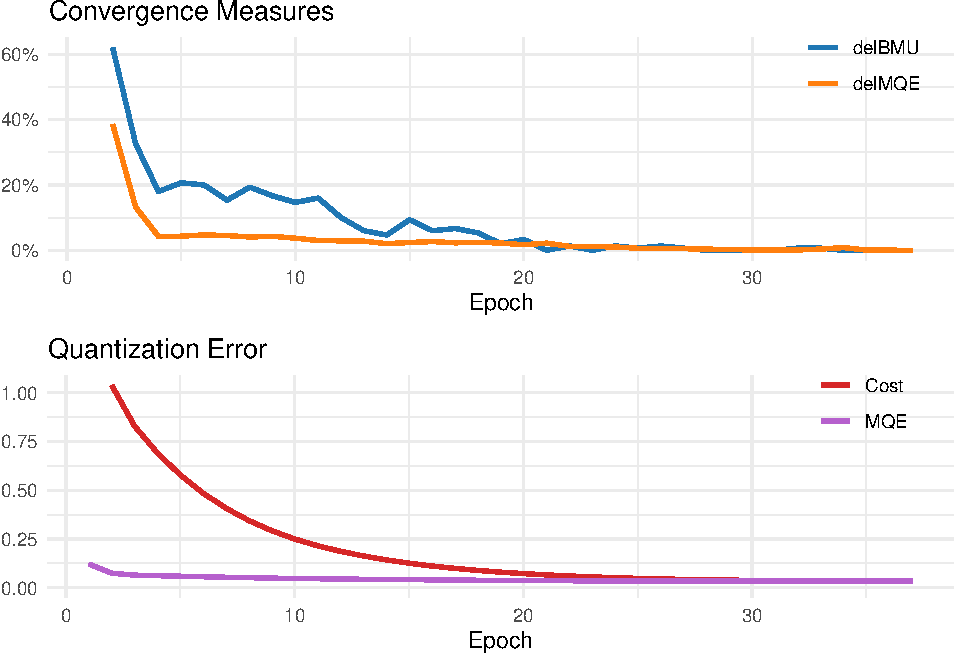
\includegraphics{NeuralGas-vignette_files/figure-latex/unnamed-chunk-5-1} \end{center}

To inspect the actual prototype placement, we can look at pairs plots of
data (gray) + prototypes (magenta) across the 4 dimensions of iris:

\begin{Shaded}
\begin{Highlighting}[]
\CommentTok{# View prototypes in data space }
\CommentTok{# First, combine the data & prototypes into one matrix for plotting }
\CommentTok{# Then specify different sizes & colors for prototype vs. data markers }
\NormalTok{pairs_data =}\StringTok{ }\KeywordTok{rbind}\NormalTok{(X, ng.iris}\OperatorTok{$}\NormalTok{W)}
\NormalTok{pairs_sizes =}\StringTok{ }\KeywordTok{c}\NormalTok{(}\KeywordTok{rep}\NormalTok{(}\FloatTok{0.5}\NormalTok{,}\KeywordTok{nrow}\NormalTok{(X)), }\KeywordTok{rep}\NormalTok{(}\FloatTok{0.75}\NormalTok{, }\KeywordTok{nrow}\NormalTok{(ng.iris}\OperatorTok{$}\NormalTok{W)))}
\NormalTok{pairs_colors =}\StringTok{ }\KeywordTok{c}\NormalTok{(}\KeywordTok{rep}\NormalTok{(}\StringTok{'darkgray'}\NormalTok{,}\KeywordTok{nrow}\NormalTok{(X)), }\KeywordTok{rep}\NormalTok{(}\StringTok{'magenta'}\NormalTok{, }\KeywordTok{nrow}\NormalTok{(ng.iris}\OperatorTok{$}\NormalTok{W)))}
\KeywordTok{pairs}\NormalTok{(pairs_data, }\DataTypeTok{cex =}\NormalTok{ pairs_sizes, }\DataTypeTok{col =}\NormalTok{ pairs_colors, }\DataTypeTok{pch=}\DecValTok{16}\NormalTok{)}
\end{Highlighting}
\end{Shaded}

\begin{center}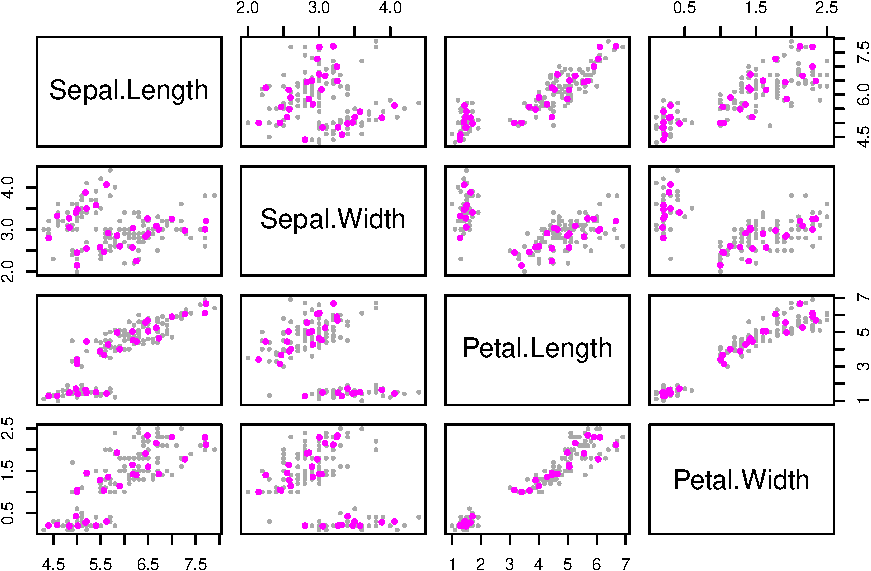
\includegraphics{NeuralGas-vignette_files/figure-latex/unnamed-chunk-6-1} \end{center}

\hypertarget{scheduled-annealing}{%
\subsection{Scheduled Annealing}\label{scheduled-annealing}}

The above learning used multiplicative decay to anneal \(\lambda\) as
training progressed. Alternatively, an annealing schedule may be
supplied as a named vector whose elements give the annealed values, and
whose names specify the epoch \textbf{through which} the respective
values are effective. For example, we can specify the following
annealing schedule
\[ \lambda(t) = \begin{cases} 7 & t \leq 1 \\ 5 & 1 < t \leq 3 \\ 3 & 3 < t \leq 5 \\ 1 & t > 5 \end{cases} \]
as a named vector \texttt{lambda\_schedule}:

\begin{Shaded}
\begin{Highlighting}[]
\CommentTok{# Define a named vector for scheduled annealing }
\NormalTok{lambda_schedule =}\StringTok{ }\KeywordTok{c}\NormalTok{(}\DecValTok{7}\NormalTok{, }\DecValTok{5}\NormalTok{, }\DecValTok{3}\NormalTok{, }\DecValTok{1}\NormalTok{)  }\CommentTok{# the desired lambda values }
\NormalTok{schedule_epochs =}\StringTok{ }\KeywordTok{c}\NormalTok{(}\DecValTok{1}\NormalTok{, }\DecValTok{3}\NormalTok{, }\DecValTok{5}\NormalTok{, }\DecValTok{6}\NormalTok{)  }\CommentTok{# the epochs after which lambda changes}
\KeywordTok{names}\NormalTok{(lambda_schedule) =}\StringTok{ }\NormalTok{schedule_epochs}
\end{Highlighting}
\end{Shaded}

The last \(\lambda\) value in the schedule will be repeated as needed if
training extends beyond \texttt{max(schedule\_epochs)} (so in this case,
\(\lambda = 1\) is used for any training epoch beyond 5). Once built (as
shown above), this schedule can be passed to the
\texttt{lambda\_schedule} argument of the \texttt{NGBatch} (or
\texttt{NGOnline}) function. If using scheduled annealing, do not supply
any values to the multliplicative annealing arguments (i.e.,
\texttt{lambda0}, \texttt{lambda\_decay}, \texttt{alpha0},
\texttt{alpha\_decay}). Checks will be performed to ensure the
scheduling occurs at integers, and that \texttt{schedule\_epochs} were
supplied in non-decreasing order. The result of learning with our
schedule specified above is:

\begin{Shaded}
\begin{Highlighting}[]
\CommentTok{# Batch learning with scheduled annealing }
\NormalTok{ng.iris.sched =}\StringTok{ }\KeywordTok{NGBatch}\NormalTok{(}\DataTypeTok{X =}\NormalTok{ X, }\DataTypeTok{W =} \KeywordTok{c}\NormalTok{(}\DecValTok{30}\NormalTok{, }\DecValTok{123}\NormalTok{), }\DataTypeTok{lambda_schedule =}\NormalTok{ lambda_schedule, }
                        \DataTypeTok{XL =}\NormalTok{ L, }\DataTypeTok{verbose =}\NormalTok{ F)}

\CommentTok{# View the LearnHist}
\KeywordTok{kbl}\NormalTok{(ng.iris.sched}\OperatorTok{$}\NormalTok{LearnHist, }\DataTypeTok{row.names =}\NormalTok{ F, }
    \DataTypeTok{digits =} \KeywordTok{c}\NormalTok{(}\DecValTok{0}\NormalTok{, }\KeywordTok{rep}\NormalTok{(}\DecValTok{3}\NormalTok{,}\DecValTok{9}\NormalTok{), }\DecValTok{0}\NormalTok{, }\DecValTok{3}\NormalTok{), }\DataTypeTok{booktabs =}\NormalTok{ T) }\OperatorTok\StringTok{ }
\StringTok{  }\KeywordTok{kable_styling}\NormalTok{(}\DataTypeTok{latex_options =} \KeywordTok{c}\NormalTok{(}\StringTok{'scale_down'}\NormalTok{,}\StringTok{"hold_position"}\NormalTok{))}
\end{Highlighting}
\end{Shaded}

\begin{table}[!h]
\centering
\resizebox{\linewidth}{!}{
\begin{tabular}[t]{rrrrrrrrrrrr}
\toprule
Epoch & lambda & Cost & MQE & NhbEff & delCost & delMQE & delBMU & Entropy & PurityWOA & WLUnq & WLHell\\
\midrule
1 & 7 & 1.848 & 0.122 & 15.176 & NaN & NaN & NaN & 0.591 & 0.893 & 3 & 0.169\\
2 & 5 & 0.668 & 0.072 & 9.331 & 63.862 & 41.228 & 66.000 & 0.775 & 0.967 & 3 & 0.069\\
3 & 5 & 0.595 & 0.059 & 10.132 & 10.990 & 18.023 & 38.000 & 0.846 & 0.973 & 3 & 0.047\\
4 & 3 & 0.280 & 0.057 & 4.925 & 52.992 & 3.300 & 19.333 & 0.891 & 0.973 & 3 & 0.054\\
5 & 3 & 0.266 & 0.050 & 5.367 & 4.921 & 12.745 & 33.333 & 0.916 & 0.973 & 3 & 0.018\\
\addlinespace
6 & 1 & 0.083 & 0.047 & 1.757 & 68.918 & 5.082 & 21.333 & 0.945 & 0.973 & 3 & 0.017\\
7 & 1 & 0.074 & 0.039 & 1.886 & 9.864 & 16.026 & 19.333 & 0.968 & 0.973 & 3 & 0.029\\
8 & 1 & 0.073 & 0.038 & 1.937 & 2.112 & 4.652 & 8.000 & 0.970 & 0.973 & 3 & 0.029\\
9 & 1 & 0.072 & 0.037 & 1.945 & 0.629 & 1.046 & 4.667 & 0.972 & 0.973 & 3 & 0.029\\
10 & 1 & 0.072 & 0.037 & 1.955 & 0.471 & 1.012 & 6.000 & 0.975 & 0.973 & 3 & 0.029\\
\addlinespace
11 & 1 & 0.072 & 0.036 & 1.971 & 0.411 & 1.188 & 5.333 & 0.976 & 0.973 & 3 & 0.029\\
12 & 1 & 0.071 & 0.036 & 1.986 & 0.409 & 1.169 & 2.000 & 0.976 & 0.973 & 3 & 0.029\\
13 & 1 & 0.071 & 0.036 & 1.992 & 0.105 & 0.397 & 0.667 & 0.975 & 0.973 & 3 & 0.029\\
14 & 1 & 0.071 & 0.036 & 1.993 & 0.048 & 0.119 & 0.667 & 0.974 & 0.973 & 3 & 0.029\\
15 & 1 & 0.071 & 0.036 & 1.995 & 0.048 & 0.137 & 0.000 & 0.974 & 0.973 & 3 & 0.029\\
\addlinespace
16 & 1 & 0.071 & 0.036 & 1.993 & 0.035 & 0.050 & 0.667 & 0.975 & 0.980 & 3 & 0.029\\
17 & 1 & 0.071 & 0.036 & 1.992 & 0.012 & 0.079 & 0.667 & 0.975 & 0.980 & 3 & 0.029\\
18 & 1 & 0.071 & 0.036 & 1.993 & 0.043 & 0.100 & 0.000 & 0.975 & 0.980 & 3 & 0.029\\
19 & 1 & 0.071 & 0.036 & 1.992 & 0.021 & 0.007 & 0.667 & 0.975 & 0.980 & 3 & 0.029\\
20 & 1 & 0.071 & 0.036 & 1.992 & 0.005 & 0.004 & 0.667 & 0.974 & 0.980 & 3 & 0.029\\
\addlinespace
21 & 1 & 0.071 & 0.036 & 1.994 & 0.048 & 0.129 & 0.000 & 0.974 & 0.980 & 3 & 0.029\\
22 & 1 & 0.071 & 0.036 & 1.994 & 0.015 & 0.006 & 0.000 & 0.974 & 0.980 & 3 & 0.029\\
23 & 1 & 0.071 & 0.036 & 1.994 & 0.006 & 0.012 & 0.000 & 0.974 & 0.980 & 3 & 0.029\\
24 & 1 & 0.071 & 0.036 & 1.994 & 0.010 & 0.027 & 0.000 & 0.974 & 0.980 & 3 & 0.029\\
\bottomrule
\end{tabular}}
\end{table}

We can see convergence occurred sooner (in 24 epochs vs.~37) with
minimal impact on final MQE (0.036 vs.~0.034).

For online learning the schedule should be set in terms of learning
iterations \(s\) (not epochs \(t\)). Additionally, if using online
learning with scheduled annealing, both \(\alpha\) and \(\lambda\) must
be scheduled (i.e., either both are scheduled, or neither). See
\texttt{NGOnline} for details.

\hypertarget{user-supplied-prototype-initializations}{%
\subsection{User-Supplied Prototype
Initializations}\label{user-supplied-prototype-initializations}}

Above we set the initial value of NG prototypes as random vectors
selected uniformaly in the range of our data. Alternatively, a user can
supply a fixed matrix of prototypes to initialize. For example,
initializing at randomly selected vectors of \(X\) is common; we show
how to achieve this below:

\begin{Shaded}
\begin{Highlighting}[]
\CommentTok{## Sample 30 vectors X to set initial prototypes }
\KeywordTok{set.seed}\NormalTok{(}\DecValTok{123}\NormalTok{)}
\NormalTok{use_these =}\StringTok{ }\KeywordTok{sample.int}\NormalTok{(}\DataTypeTok{n =} \KeywordTok{nrow}\NormalTok{(X), }\DataTypeTok{size =} \DecValTok{30}\NormalTok{, }\DataTypeTok{replace =}\NormalTok{ F)}
\NormalTok{W0 =}\StringTok{ }\NormalTok{X[use_these,]}

\CommentTok{## Train with default lambda and annealing }
\NormalTok{ng.iris =}\StringTok{ }\KeywordTok{NGBatch}\NormalTok{(}\DataTypeTok{X =}\NormalTok{ X, }\DataTypeTok{W =}\NormalTok{ W0, }\DataTypeTok{XL =}\NormalTok{ L, }\DataTypeTok{verbose =}\NormalTok{ F)}
\KeywordTok{str}\NormalTok{(ng.iris)}
\CommentTok{## List of 12}
\CommentTok{##  $ W              : num [1:30, 1:4] 4.82 5.34 7.69 4.4 6.76 ...}
\CommentTok{##  $ epochs         : num 35}
\CommentTok{##  $ lambda_start   : num 7.5}
\CommentTok{##  $ lambda_end     : num 0.209}
\CommentTok{##  $ lambda_decay   : num 0.9}
\CommentTok{##  $ lambda_schedule: NULL}
\CommentTok{##  $ tol_delBMU     : num 1}
\CommentTok{##  $ tol_delMQE     : num 0.1}
\CommentTok{##  $ max_epochs     : int 999999}
\CommentTok{##  $ exec_time      : num 8.54e-05}
\CommentTok{##  $ converged      : logi TRUE}
\CommentTok{##  $ LearnHist      :'data.frame': 35 obs. of  12 variables:}
\CommentTok{##   ..$ Epoch    : num [1:35] 1 2 3 4 5 6 7 8 9 10 ...}
\CommentTok{##   ..$ lambda   : num [1:35] 7.5 6.75 6.08 5.47 4.92 ...}
\CommentTok{##   ..$ Cost     : num [1:35] 1.226 0.975 0.819 0.688 0.577 ...}
\CommentTok{##   ..$ MQE      : num [1:35] 0.0395 0.0718 0.0649 0.0624 0.0597 ...}
\CommentTok{##   ..$ NhbEff   : num [1:35] 31.02 13.59 12.63 11.03 9.67 ...}
\CommentTok{##   ..$ delCost  : num [1:35] NaN 20.4 16 16 16.1 ...}
\CommentTok{##   ..$ delMQE   : num [1:35] NaN 81.59 9.59 3.89 4.26 ...}
\CommentTok{##   ..$ delBMU   : num [1:35] NaN 77.3 30 19.3 20.7 ...}
\CommentTok{##   ..$ Entropy  : num [1:35] 0.956 0.826 0.847 0.873 0.89 ...}
\CommentTok{##   ..$ PurityWOA: num [1:35] 0.967 0.947 0.96 0.967 0.973 ...}
\CommentTok{##   ..$ WLUnq    : num [1:35] 3 3 3 3 3 3 3 3 3 3 ...}
\CommentTok{##   ..$ WLHell   : num [1:35] 0.0289 0.1609 0.1282 0.0776 0.0681 ...}
\end{Highlighting}
\end{Shaded}





\newpage
\singlespacing 
\printbibliography

\end{document}